There has been several previous and related works that attempted to parallelize and improve on serial implementations of the aforementioned minimax algorithm.\cite{borovska} \cite{Rocki} \cite{Mandadi}.\\
\\
Rocki and Suda explored CUDA-implemented parallel minimax tree search for Othello. This work was particularly important for this work as it highlighted some of the challenges of naive GPU implementations like thread divergence. Optimizations to the naive implementation that they propose like the sequential-parallel CUDA search are included in this work and will be explained further in detail in Section~\ref{sec:gpu}. \cite{Rocki}\\
\\
Borovska and Lazarova similarly explored parallel implementations of the minimax algorithm, but for tic-tac-toe. However, the parallelism that they expose is slightly different compared to Rocki and Suda and they describe them as \textit{partitioning at width} and \textit{partitioning at depth}, where \textit{partitioning at width} describes Rocki and Suda's approach and \textit{partitioning at depth} describes Borovska and Lazarova's approach. Figure~\ref{fig:widthvdepth} graphically shows the distinction that they draw. The \textit{partitioning at width} approach that Rocki and Suda take is to simply assign the search tree and assign them to multiple processors/threads for processing. The \textit{partitioning at width} approach that Borovska and Lazarova take is an attempt to leverage parallelism while keeping the benefits of alpha-beta pruning alive by instead parallelizing the move evaluation at each depth. They implement this with MPI and achieves around 2x speedup compared to serial code. It should be noted here though that tic-tac-toe is significantly less complex as a game compared to Gomoku. The PVS CUDA implementation described in Section~\ref{sec:gpu} will build off of this parallelization strategy.\cite{borovska}.


\begin{figure}[!htbp]
    \centering
    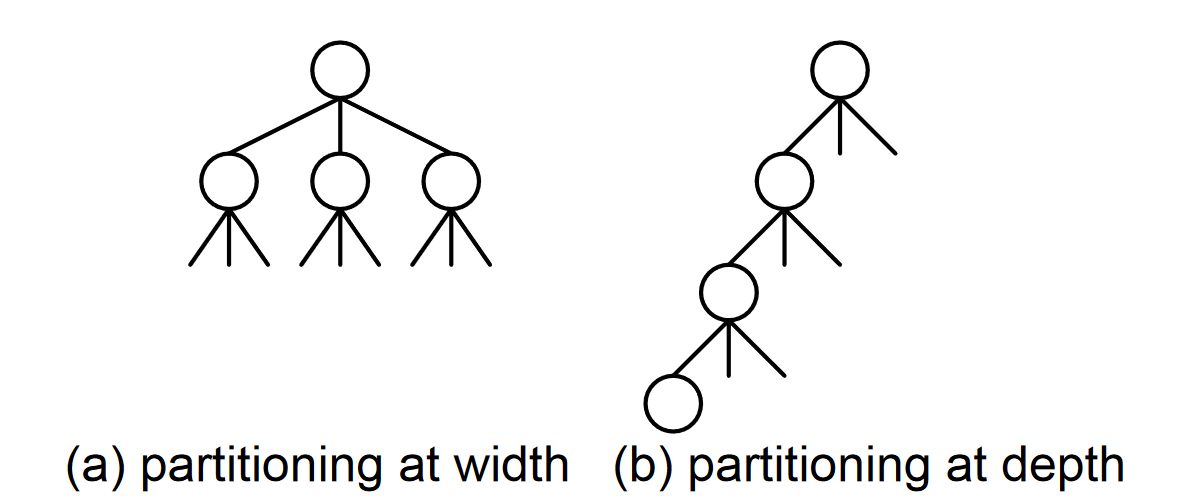
\includegraphics[scale=0.3]{images/relwork1.PNG}
    \caption{Partitioning at width vs depth}
    \label{fig:widthvdepth}
\end{figure}

